\documentclass[prb,12pt]{revtex4-2}

\usepackage{amsmath, amssymb,physics,amsfonts,amsthm}
\usepackage{enumitem}
\usepackage[most]{tcolorbox}
\usepackage{cancel}
\usepackage{booktabs}
\usepackage{tikz}
\usepackage{hyperref}
\usepackage{enumitem}
\usepackage{tabularx}
\usepackage[ngerman]{babel}
\usepackage{transparent}
\usepackage{float}
\usepackage{multirow}
\usepackage{bbm}
%\usepackage{subcaption}
\usepackage{longtable}
%code
\usepackage{listings}
\usepackage{xcolor} 
\definecolor{listinggray}{gray}{0.9}
\definecolor{lbcolor}{rgb}{0.9,0.9,0.9}
\definecolor{Darkgreen}{rgb}{0,0.4,0}
\lstset{
	backgroundcolor=\color{lbcolor},
	tabsize=4,    
	%   rulecolor=,
	language=[GNU]C++,
	basicstyle=\scriptsize,
	upquote=true,
	aboveskip={1.5\baselineskip},
	columns=fixed,
	showstringspaces=false,
	extendedchars=false,
	breaklines=true,
	prebreak = \raisebox{0ex}[0ex][0ex]{\ensuremath{\hookleftarrow}},
	frame=single,
	numbers=left,
	showtabs=false,
	showspaces=false,
	showstringspaces=false,
	identifierstyle=\ttfamily,
	keywordstyle=\color[rgb]{0,0,1},
	commentstyle=\color[rgb]{0.026,0.112,0.095},
	stringstyle=\color[rgb]{0.627,0.126,0.941},
	numberstyle=\color[rgb]{0.205, 0.142, 0.73},
	%        \lstdefinestyle{C++}{language=C++,style=numbers}’.
}
\lstset{
	backgroundcolor=\color{lbcolor},
	tabsize=4,
	language=C++,
	captionpos=b,
	tabsize=3,
	frame=lines,
	numbers=left,
	numberstyle=\tiny,
	numbersep=5pt,
	breaklines=true,
	showstringspaces=false,
	basicstyle=\footnotesize,
	%  identifierstyle=\color{magenta},
	keywordstyle=\color[rgb]{0,0,1},
	commentstyle=\color{Darkgreen},
	stringstyle=\color{red}
}

\newtheorem{Theorem}{Theorem}
\newtheorem{Proposition}{Theorem}
\newtheorem{Lemma}[Theorem]{Lemma}
\newtheorem{Corollary}[Theorem]{Corollary}
\newtheorem{Example}[Theorem]{Example}
\newtheorem{Remark}[Theorem]{Remark}
\theoremstyle{definition}
\newtheorem{Problem}{Problem}
\theoremstyle{definition}
\newtheorem{Definition}[Theorem]{Definition}
\newenvironment{parts}{\begin{enumerate}[label=(\alph*)]}{\end{enumerate}}
%tikz	
\tcbset{breakable=true,toprule at break = 0mm,bottomrule at break = 0mm}
\usetikzlibrary{patterns}
\usetikzlibrary{matrix}
\usepackage{pgfplots}
\pgfplotsset{compat=1.18}
% definitions of number sets
\newcommand{\N}{\mathbb{N}}
\newcommand{\R}{\mathbb{R}}
\newcommand{\Z}{\mathbb{Z}}
\newcommand{\Q}{\mathbb{Q}}
\newcommand{\C}{\mathbb{C}}
\allowdisplaybreaks
\begin{document}
\title{Statistische Mechanik Bonusblatt}
	\author{Jun Wei Tan}
	\email{jun-wei.tan@stud-mail.uni-wuerzburg.de}
	\affiliation{Julius-Maximilians-Universit\"{a}t W\"{u}rzburg}
	\date{\today}
	\maketitle
\tableofcontents

\section{Aufgabe 1}
Betrachten Sie eine Kette aus \( N \) Monomeren der Größe \( a \) in zwei Dimensionen. D.h., jedem Glied \( i \) kann der Vektor \( \vec{r}_i \) zugeordnet werden, der in eine beliebige Richtung zeigen kann und die Länge \( |\vec{r}_i| = a \) hat.

\begin{enumerate}
	\item[a)] Berechnen Sie für dieses System die mittlere quadratische Distanz zwischen Anfangs- und Endpunkt:
	\[
	\langle \vec{R}^2 \rangle = \left\langle \left( \sum_{i=1}^N \vec{r}_i \right)^2 \right\rangle
	\]
	\textit{Hinweis: Hier lässt sich mit Symmetrie argumentieren. Was ist \( \langle \vec{r}_i \cdot \vec{r}_j \rangle \) für \( i = j \) bzw. für \( i \neq j \)?}
	
	\item[b)] Das Polymer befindet sich jetzt in einem Wärmebad mit der Temperatur \( T \). Die beiden Enden des Polymers werden mit einer Kraft \( \vec{F} = (0, 0, F) \) auseinandergezogen, so dass \((1)\) gilt. Berechnen Sie die Korrelationsfunktionen
	\[
	\langle \vec{R} \rangle = \left\langle \sum_{i=1}^N \vec{r}_i \right\rangle,
	\]
	\[
	\langle \vec{R}^2 \rangle = \left\langle \left( \sum_{i=1}^N \vec{r}_i \right)^2 \right\rangle
	\]
	als Funktion der Kraft und der Temperatur. Wie verhalten sich diese in den Grenzfällen \( aF \ll k_B T \) und \( aF \gg k_B T \)?
\end{enumerate}
\begin{proof}
	\begin{enumerate}[label=\alph*)]
		\item Für $i\neq j$ sind $\vec{r}_i$ und $\vec{r}_j$ unabhängig. Damit ist
		\[\langle \vec{r}_i \cdot \vec{r}_j\rangle = \langle \vec{r}_i\rangle \cdot \langle \vec{r}_j\rangle = \vec{0}\cdot \vec{0}=0.\]
		F\"{u}r $i=j$ ist $\vec{r}_i\cdot \vec{r}_j= |\vec{r}_i|^2=a^2$, was überhaupt nicht stochastisch ist und damit ist $\langle \vec{r}_i \cdot \vec{r}_i\rangle = a^2$. Damit ist
		\begin{align*}
			\langle \vec{R}^2 \rangle &= \left\langle \left( \sum_{i=1}^N \vec{r}_i \right)^2 \right\rangle \\
			&= \left\langle \sum_{i=1}^N \sum_{j=1}^N \vec{r}_i \cdot \vec{r}_j \right\rangle\\
			&=\sum_{i=1}^N \sum_{j=1}^N \langle \vec{r}_i \cdot \vec{r}_j \rangle\\
			&=\sum_{i=1}^N \sum_{j=1}^N a^2 \delta_{ij}\\
			&= Na^2.
		\end{align*}
	\end{enumerate}
\item Die kanonische Zustandssumme ist
\[Z = \int_{S^2} \dots \int_{S^2} \exp\left(-\beta H\right)\dd{\vec{r}_i}\dots \dd{\vec{r}_n}\]
wobei $S^2$ der Einheitskreis in 3-Dim und
\[H = -\sum_{i=1}^n \vec{F}\cdot \vec{r}_i\]
ist. Damit gilt
\[
	Z = \int_{S^2}\dots \int_{S^2} \prod_{k=1}^n e^{\beta \vec{F}\cdot\vec{r}_k} \dd{\vec{r}_1} \dots \dd{\vec{r}_n}.\]
	Ein inneres Integral ist
	\begin{align*}
		\int_{S^2} e^{\beta(\vec{F}\cdot \vec{r})}\dd{\vec{r}} &= \int_0^{2\pi}\int_0^{\pi} e^{\beta F a \cos \theta}\sin\theta \dd{\theta}\dd{\varphi}\\
		&=-2\pi \int_1^{-1} e^{\beta F a u}\dd{u}\\
		&=\frac{4\pi \sinh (a F \beta)}{a F \beta}
	\end{align*}
und damit ist
\[Z = \left[\frac{4\pi \sinh (a F \beta)}{a F \beta}\right]^N.\]
Nun bestimmen wir die 3 Komponente des Vektors $\langle \vec{R}\rangle$ $\langle R_i\rangle$. Es gilt
\begin{align*}
	\langle R_i \rangle &= \frac 1Z \int_{(S^2)^n} R_i \exp\left(\beta \sum_{k=1}^n \sum_{p\in \{x,y,z\}} F_p (r_k)_p\right)\dd{\vec{r}_1}\dots \dd{\vec{r}_n}\\
	&= \frac 1Z \int_{(S^2)^n} \left(\sum_{l=1}^n (r_l)_i\right) \exp\left(\beta \sum_{k=1}^n \sum_{p\in \{x,y,z\}} F_p (r_k)_p\right)\dd{\vec{r}_1}\dots \dd{\vec{r}_n}\\
	&=\frac 1\beta \frac 1Z \int_{(S^2)^n} \pdv{F_i} \exp\left(\beta \sum_{k=1}^n \sum_{p\in \{x,y,z\}} F_p (r_k)_p\right)\dd{\vec{r}_1}\dots \dd{\vec{r}_n}\\
	&= \frac 1\beta \pdv{F_i}\ln Z
\end{align*}
In diesem Fall hat $F$ nur eine $z$-Komponente. Damit verschwinden die $x$ und $y$ Ableitungen:
\[\langle R_x \rangle = \langle R_y \rangle = 0.\]
Die $z$-Komponente ist
\begin{align*}
	\langle R_z \rangle &= \frac 1\beta \pdv{F} N \ln \frac{4\pi \sinh (a F \beta)}{a F \beta}\\
	&=\frac{N}{\beta} \left[a \beta  \coth (a \beta  F)-\frac{1}{F}\right]\\
	&=Na \coth (a \beta F) - \frac{N}{\beta F}.
\end{align*}
Zur Bestimmung von $\langle R^2\rangle$ betrachten wir
\begin{align*}
	\langle R^2\rangle &= \frac 1Z \int_{(S^2)^N} R^2 \exp\left(\beta \sum_{k=1}^N \sum_{p\in \{x,y,z\}} F_p (r_k)_p\right)\dd{\vec{r}_1}\dots \dd{\vec{r}_N}\\
	&=  \frac 1Z \int_{(S^2)^N}  \sum_{i\in \{x,y,z\}}\left(\sum_{l=1}^N (r_l)_i\right)^2  \exp\left(\beta \sum_{k=1}^N \sum_{p\in \{x,y,z\}} F_p (r_k)_p\right)\dd{\vec{r}_1}\dots \dd{\vec{r}_N}\\
	&= \frac 1Z \int_{(S^2)^N}  \sum_{i\in \{x,y,z\}}\frac{1}{\beta^2}\pdv[2]{F_i} \exp\left(\beta \sum_{k=1}^N \sum_{p\in \{x,y,z\}} F_p (r_k)_p\right)\dd{\vec{r}_1}\dots \dd{\vec{r}_N}\\
	&= \frac 1Z \frac{1}{\beta^2}\sum_{i\in \{x,y,z\}}\pdv[2]{Z}{F_i}.
\end{align*}
Die Ableitungen nach $F_x$ und $F_y$ verschwinden wieder und damit bleibt nur
\begin{align*}
\langle R^2\rangle &= \frac 1{\beta^2 Z}\pdv[2]{Z}{F}\\
&=\frac{N (4 \pi )^N\left(a^2 \beta ^2 F^2+a^2 \beta ^2 F^2 (N-1) \coth ^2(a \beta  F)-2 a \beta  F N \coth (a \beta  F)+N+1\right)}{F^2\beta^2}.\qedhere
\end{align*}
\end{proof}
\section{Aufgabe 2}
Die Codes befinden sich im Anhang \ref{sec:code}. Die sind für den Random Walk und den Self Avoiding Random Walk zwar sehr ähnlich, können aber nicht vertauscht werden, da die Methode \texttt{generateWalk()} unterschiedlich implementiert wird. Beim SARW unterbricht die Methode, sobald die Trajektorie sich schneidet. Damit spart das Programm $O(1)$ Zeit, was die Zeitkomplexität jedoch nicht ändert. Mit der Flagge -O3 läuft das Programm für den RW in 5.146s und das Programm für den SARW in 141.988s.

\begin{figure}[H]
	\centering
	\includegraphics[width=0.4\textwidth]{your did it.jpeg}
	\caption{Ich, nachdem mein Code 0.01\% schneller läuft.}
\end{figure}

20 Trajektorien für den RW und den SARW sind in Abb. \ref{fig:trajectories} dargestellt. Ein Best-Fit-Gerade wurde zu den Daten im Anhang \ref{sec:data} bestimmt. F\"{u}r den Random-Walk ist es aus den Daten klar, dass eine lineare Anpassung sehr gut geeignet ist. Damit führen wir eine lineare Regression durch. F\"{u}r den SARW f\"{u}hren wir stattdessen eine lineare Regression in log-log Skala bzw. eine polynomiale Anpassung durch.

Damit ist die lineare Anpassung zum RW (geplottet in Abb. \ref{fig:plots}(a)):
\[y = a + bx\]
mit Parameter
\begin{align*}
	a &= 0.052\pm 0.010\\
	b &= 1.000241\pm 0.000088
\end{align*}
Weil der RW noch symmetrisch ist, können wir dasselbe Argument wie in Aufgabe 1a anwende. Es ist also zu erwarten, dass $\langle R^2(t)\rangle = t$. Dies stimmt nicht im Rahmen des Fehlers mit der Regressionsgerade überein. Es liegt wahrscheinlich daran, dass die $\langle R(t)^2\rangle$ zu unterschiedlichen Zeitpunkten korreliert sind. Dies sieht man in Abb. \ref{fig:plots}(b). Wenn die Werte unabhängig wären, wäre die Streuung symmetrisch oberhalb und unterhalb der $x=y$ Gerade. Stattdessen sieht man eine kontinuierliche Kurve. Die Korrelation sieht man durch ein Beispiel: Wenn eine Kette weiter weg vom Ursprung als erwartet wandert, werden die folgenden Abstände auch größer als erwartet. Damit führt eine kleine statistische Abweichung am Anfang zu einer fortgesetzten Abweichung in der gleichen Richtung, was die Parameter der Regression ändern kann.

F\"{u}r den SARW machen wir stattdessen eine polynomiale Anpassung (Abb. \ref{fig:plots}(c))
\[y = A x^b\]
mit Parameter
\begin{align*}
	A &= 0.9820\pm 0.0059\\
	b &=1.4603\pm 0.0024
\end{align*}
Es ist auffällig, dass die letzten 3 Punkte nicht an der Gerade liegen. Es liegt vermutlich daran, dass die Verteilung von der Länge abhängig ist. Es kann sein, dass manche Pfade sich verschließen. Dann wäre dieser Pfad abgelehnt, wenn er fortgesetzt wäre. Daher gibt es auch den Begriff des Non-Trapped Self Avoiding Walks. Da unser Programm bei einer endlichen Anzahl von Schritte haltet, sind diese Pfade aber nicht abgelehnt. Dies führt zu einer geringen Abstand vom Ursprung als erwartet, was wir im Ergebnis sehen. 

Der Abstand vom Ursprung steigt schneller für den SARW als für den RW. Weil die Pfade nicht selbst schneiden können, gibt es immer ein Bereich um Ursprung, der \glqq verboten\grqq~  ist. Damit ist die Wahrscheinlichkeit größer, dass der Pfad weg vom Ursprung wandert. 
\begin{figure*}
	\centering
	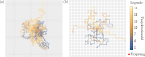
\includegraphics[width=0.8\textwidth]{fig1.pdf}
	\caption{20 Trajektorien sind dargestellt. \textbf{(a)} Trajektorien des Random Walks mit L\"{a}nge 200. \textbf{(b)} Trajektorien des Self Avoiding Random Walks mit L\"{a}nge 30. }
	\label{fig:trajectories}
\end{figure*}
\begin{figure*}
	\centering
	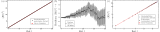
\includegraphics[width=\textwidth]{fig2.pdf}
	\caption{\textbf{(a)} Durchschnittlicher quadratischer Abstand des RWs vom Ursprung in Abhängigkeit von der Zeit bzw. Anzahl der Schritte. Die lineare Anpassung $y=0.052 + 1.000241x$ stimmt sehr gut mit den Daten überein. \textbf{(b)} Residuen bezüglich der Gerade $y=x$. Die Residuen zu unterschiedlichen Zeitpunkten sind korreliert. \textbf{(c)} Durchschnittlicher quadratischer Abstand des SARWs in Abhängigkeit der Zeit in log-log Skala. Eine Gerade wird zu den ersten 27 Punkten angepasst.}
	\label{fig:plots}
\end{figure*}

\appendix
\section{Code}\label{sec:code}
\subsection{Code für den Random Walk}
\lstinputlisting{../main.cpp}
\subsection{Code für den Self Avoiding Random Walk}
\lstinputlisting{../mainAvoiding.cpp}
\section{Simulationsdaten}\label{sec:data}
\subsection{Daten für den Random Walk}
\begin{longtable}{cc}
	\toprule
	Zeit ($t$) & $\langle R(t)^2 \rangle $\\\midrule
 0 & $0\pm 0$ \\\midrule
1 & $1\pm 0$ \\\midrule
2 & $1.9995\pm 0.0014$ \\\midrule
3 & $2.9973\pm 0.0024$ \\\midrule
4 & $3.9984\pm 0.0035$ \\\midrule
5 & $5.0028\pm 0.0045$ \\\midrule
6 & $6.0034\pm 0.0055$ \\\midrule
7 & $7.0019\pm 0.0065$ \\\midrule
8 & $8.0022\pm 0.0075$ \\\midrule
9 & $8.9991\pm 0.0085$ \\\midrule
10 & $10.0009\pm 0.0095$ \\\midrule
11 & $11.001\pm 0.010$ \\\midrule
12 & $11.995\pm 0.011$ \\\midrule
13 & $12.996\pm 0.012$ \\\midrule
14 & $13.995\pm 0.013$ \\\midrule
15 & $15.001\pm 0.014$ \\\midrule
16 & $16.000\pm 0.015$ \\\midrule
17 & $17.002\pm 0.016$ \\\midrule
18 & $18.001\pm 0.017$ \\\midrule
19 & $18.998\pm 0.019$ \\\midrule
20 & $20.008\pm 0.020$ \\\midrule
21 & $21.008\pm 0.021$ \\\midrule
22 & $22.015\pm 0.022$ \\\midrule
23 & $23.015\pm 0.023$ \\\midrule
24 & $24.018\pm 0.024$ \\\midrule
25 & $25.015\pm 0.025$ \\\midrule
26 & $26.009\pm 0.026$ \\\midrule
27 & $27.006\pm 0.027$ \\\midrule
28 & $28.020\pm 0.028$ \\\midrule
29 & $29.015\pm 0.029$ \\\midrule
30 & $30.014\pm 0.030$ \\\midrule
31 & $31.012\pm 0.030$ \\\midrule
32 & $32.016\pm 0.031$ \\\midrule
33 & $33.012\pm 0.032$ \\\midrule
34 & $34.017\pm 0.033$ \\\midrule
35 & $35.025\pm 0.034$ \\\midrule
36 & $36.014\pm 0.035$ \\\midrule
37 & $37.006\pm 0.036$ \\\midrule
38 & $38.013\pm 0.037$ \\\midrule
39 & $39.016\pm 0.038$ \\\midrule
40 & $40.025\pm 0.039$ \\\midrule
41 & $41.057\pm 0.041$ \\\midrule
42 & $42.051\pm 0.042$ \\\midrule
43 & $43.034\pm 0.043$ \\\midrule
44 & $44.038\pm 0.044$ \\\midrule
45 & $45.041\pm 0.045$ \\\midrule
46 & $46.049\pm 0.046$ \\\midrule
47 & $47.043\pm 0.047$ \\\midrule
48 & $48.050\pm 0.048$ \\\midrule
49 & $49.063\pm 0.049$ \\\midrule
50 & $50.050\pm 0.050$ \\\midrule
51 & $51.047\pm 0.051$ \\\midrule
52 & $52.051\pm 0.052$ \\\midrule
53 & $53.052\pm 0.053$ \\\midrule
54 & $54.054\pm 0.054$ \\\midrule
55 & $55.059\pm 0.055$ \\\midrule
56 & $56.053\pm 0.056$ \\\midrule
57 & $57.041\pm 0.057$ \\\midrule
58 & $58.049\pm 0.058$ \\\midrule
59 & $59.052\pm 0.059$ \\\midrule
60 & $60.054\pm 0.060$ \\\midrule
61 & $61.072\pm 0.061$ \\\midrule
62 & $62.049\pm 0.062$ \\\midrule
63 & $63.044\pm 0.063$ \\\midrule
64 & $64.047\pm 0.064$ \\\midrule
65 & $65.061\pm 0.065$ \\\midrule
66 & $66.065\pm 0.066$ \\\midrule
67 & $67.062\pm 0.067$ \\\midrule
68 & $68.075\pm 0.068$ \\\midrule
69 & $69.090\pm 0.069$ \\\midrule
70 & $70.092\pm 0.070$ \\\midrule
71 & $71.089\pm 0.071$ \\\midrule
72 & $72.089\pm 0.072$ \\\midrule
73 & $73.096\pm 0.073$ \\\midrule
74 & $74.084\pm 0.074$ \\\midrule
75 & $75.091\pm 0.075$ \\\midrule
76 & $76.074\pm 0.076$ \\\midrule
77 & $77.064\pm 0.077$ \\\midrule
78 & $78.091\pm 0.078$ \\\midrule
79 & $79.105\pm 0.079$ \\\midrule
80 & $80.119\pm 0.080$ \\\midrule
81 & $81.120\pm 0.081$ \\\midrule
82 & $82.124\pm 0.082$ \\\midrule
83 & $83.100\pm 0.083$ \\\midrule
84 & $84.111\pm 0.084$ \\\midrule
85 & $85.100\pm 0.085$ \\\midrule
86 & $86.100\pm 0.086$ \\\midrule
87 & $87.086\pm 0.087$ \\\midrule
88 & $88.083\pm 0.088$ \\\midrule
89 & $89.113\pm 0.089$ \\\midrule
90 & $90.121\pm 0.090$ \\\midrule
91 & $91.124\pm 0.091$ \\\midrule
92 & $92.135\pm 0.092$ \\\midrule
93 & $93.143\pm 0.093$ \\\midrule
94 & $94.149\pm 0.094$ \\\midrule
95 & $95.145\pm 0.095$ \\\midrule
96 & $96.135\pm 0.096$ \\\midrule
97 & $97.141\pm 0.097$ \\\midrule
98 & $98.137\pm 0.098$ \\\midrule
99 & $99.132\pm 0.099$ \\\midrule
100 & $100.149\pm 0.10$ \\\midrule
101 & $101.15\pm 0.10$ \\\midrule
102 & $102.15\pm 0.10$ \\\midrule
103 & $103.15\pm 0.10$ \\\midrule
104 & $104.17\pm 0.10$ \\\midrule
105 & $105.16\pm 0.10$ \\\midrule
106 & $106.16\pm 0.11$ \\\midrule
107 & $107.17\pm 0.11$ \\\midrule
108 & $108.16\pm 0.11$ \\\midrule
109 & $109.18\pm 0.11$ \\\midrule
110 & $110.17\pm 0.11$ \\\midrule
111 & $111.14\pm 0.11$ \\\midrule
112 & $112.13\pm 0.11$ \\\midrule
113 & $113.13\pm 0.11$ \\\midrule
114 & $114.15\pm 0.11$ \\\midrule
115 & $115.15\pm 0.11$ \\\midrule
116 & $116.17\pm 0.12$ \\\midrule
117 & $117.18\pm 0.12$ \\\midrule
118 & $118.18\pm 0.12$ \\\midrule
119 & $119.19\pm 0.12$ \\\midrule
120 & $120.18\pm 0.12$ \\\midrule
121 & $121.21\pm 0.12$ \\\midrule
122 & $122.23\pm 0.12$ \\\midrule
123 & $123.24\pm 0.12$ \\\midrule
124 & $124.21\pm 0.12$ \\\midrule
125 & $125.24\pm 0.12$ \\\midrule
126 & $126.23\pm 0.13$ \\\midrule
127 & $127.25\pm 0.13$ \\\midrule
128 & $128.24\pm 0.13$ \\\midrule
129 & $129.22\pm 0.13$ \\\midrule
130 & $130.22\pm 0.13$ \\\midrule
131 & $131.21\pm 0.13$ \\\midrule
132 & $132.19\pm 0.13$ \\\midrule
133 & $133.16\pm 0.13$ \\\midrule
134 & $134.15\pm 0.13$ \\\midrule
135 & $135.17\pm 0.13$ \\\midrule
136 & $136.17\pm 0.14$ \\\midrule
137 & $137.17\pm 0.14$ \\\midrule
138 & $138.17\pm 0.14$ \\\midrule
139 & $139.14\pm 0.14$ \\\midrule
140 & $140.17\pm 0.14$ \\\midrule
141 & $141.14\pm 0.14$ \\\midrule
142 & $142.13\pm 0.14$ \\\midrule
143 & $143.16\pm 0.14$ \\\midrule
144 & $144.18\pm 0.14$ \\\midrule
145 & $145.19\pm 0.14$ \\\midrule
146 & $146.19\pm 0.15$ \\\midrule
147 & $147.19\pm 0.15$ \\\midrule
148 & $148.17\pm 0.15$ \\\midrule
149 & $149.15\pm 0.15$ \\\midrule
150 & $150.12\pm 0.15$ \\\midrule
151 & $151.14\pm 0.15$ \\\midrule
152 & $152.11\pm 0.15$ \\\midrule
153 & $153.09\pm 0.15$ \\\midrule
154 & $154.10\pm 0.15$ \\\midrule
155 & $155.12\pm 0.15$ \\\midrule
156 & $156.11\pm 0.16$ \\\midrule
157 & $157.10\pm 0.16$ \\\midrule
158 & $158.07\pm 0.16$ \\\midrule
159 & $159.09\pm 0.16$ \\\midrule
160 & $160.09\pm 0.16$ \\\midrule
161 & $161.09\pm 0.16$ \\\midrule
162 & $162.07\pm 0.16$ \\\midrule
163 & $163.08\pm 0.16$ \\\midrule
164 & $164.06\pm 0.16$ \\\midrule
165 & $165.02\pm 0.16$ \\\midrule
166 & $166.01\pm 0.17$ \\\midrule
167 & $166.98\pm 0.17$ \\\midrule
168 & $167.99\pm 0.17$ \\\midrule
169 & $169.00\pm 0.17$ \\\midrule
170 & $170.00\pm 0.17$ \\\midrule
171 & $171.00\pm 0.17$ \\\midrule
172 & $171.97\pm 0.17$ \\\midrule
173 & $172.95\pm 0.17$ \\\midrule
174 & $173.95\pm 0.17$ \\\midrule
175 & $174.98\pm 0.17$ \\\midrule
176 & $175.98\pm 0.18$ \\\midrule
177 & $176.98\pm 0.18$ \\\midrule
178 & $177.97\pm 0.18$ \\\midrule
179 & $178.99\pm 0.18$ \\\midrule
180 & $179.98\pm 0.18$ \\\midrule
181 & $181.00\pm 0.18$ \\\midrule
182 & $182.01\pm 0.18$ \\\midrule
183 & $183.02\pm 0.18$ \\\midrule
184 & $184.00\pm 0.18$ \\\midrule
185 & $184.99\pm 0.18$ \\\midrule
186 & $185.99\pm 0.19$ \\\midrule
187 & $186.98\pm 0.19$ \\\midrule
188 & $188.01\pm 0.19$ \\\midrule
189 & $189.01\pm 0.19$ \\\midrule
190 & $190.03\pm 0.19$ \\\midrule
191 & $191.02\pm 0.19$ \\\midrule
192 & $192.03\pm 0.19$ \\\midrule
193 & $193.00\pm 0.19$ \\\midrule
194 & $194.00\pm 0.19$ \\\midrule
195 & $195.00\pm 0.19$ \\\midrule
196 & $195.99\pm 0.20$ \\\midrule
197 & $197.00\pm 0.20$ \\\midrule
198 & $198.05\pm 0.20$ \\\midrule
199 & $199.04\pm 0.20$ \\\midrule
200 & $200.00\pm 0.20$ \\\bottomrule
\end{longtable}
\subsection{Daten für den Self Avoiding Random Walk}
\begin{longtable}{cc}
	\toprule
	Zeit ($t$) & $\langle R(t)^2 \rangle $\\\midrule
 0 & $0\pm 0$ \\\midrule
1 & $1\pm 0$ \\\midrule
2 & $2.7046\pm 0.0096$ \\\midrule
3 & $4.798\pm 0.022$ \\\midrule
4 & $7.388\pm 0.035$ \\\midrule
5 & $10.232\pm 0.051$ \\\midrule
6 & $13.376\pm 0.069$ \\\midrule
7 & $16.752\pm 0.088$ \\\midrule
8 & $20.33\pm 0.11$ \\\midrule
9 & $24.12\pm 0.13$ \\\midrule
10 & $28.30\pm 0.16$ \\\midrule
11 & $32.61\pm 0.18$ \\\midrule
12 & $36.96\pm 0.21$ \\\midrule
13 & $41.62\pm 0.23$ \\\midrule
14 & $46.45\pm 0.26$ \\\midrule
15 & $51.49\pm 0.29$ \\\midrule
16 & $56.75\pm 0.33$ \\\midrule
17 & $62.18\pm 0.36$ \\\midrule
18 & $67.72\pm 0.39$ \\\midrule
19 & $73.24\pm 0.42$ \\\midrule
20 & $78.87\pm 0.46$ \\\midrule
21 & $84.67\pm 0.49$ \\\midrule
22 & $90.22\pm 0.53$ \\\midrule
23 & $95.88\pm 0.56$ \\\midrule
24 & $101.55\pm 0.60$ \\\midrule
25 & $107.18\pm 0.64$ \\\midrule
26 & $112.70\pm 0.68$ \\\midrule
27 & $118.05\pm 0.72$ \\\midrule
28 & $122.96\pm 0.76$ \\\midrule
29 & $127.14\pm 0.80$ \\\midrule
30 & $130.25\pm 0.84$ \\\bottomrule
\end{longtable}
\end{document}
